\documentclass{book}

\usepackage{subcaption}
\usepackage{longtable}
\usepackage{xcolor}
\usepackage{geometry}
\usepackage{ragged2e}
\usepackage{float}
\usepackage{listings}
\usepackage{caption}
\usepackage{hyperref}
\usepackage{titlesec}
\usepackage{graphicx}
\usepackage{amsmath}
\usepackage{fmtcount}
\usepackage{fancyhdr}
\usepackage{lipsum}
\usepackage{wrapfig}
\usepackage{tikz}
\usetikzlibrary{shapes,arrows,positioning}
\usepackage[most]{tcolorbox}
\usepackage{xurl}

\usepackage[T1]{fontenc}
\usepackage[utf8]{inputenc}
\usepackage[english]{babel}

\begin{document}
\title{Projek kontrolera lotu}
\author{Krzysztof Jamrozy}
\date{}

\maketitle
% color style define for code listing
\definecolor{comments}{rgb}{0.94,0.45,0.36}
\definecolor{black_numbers}{rgb}{0.08,0.1,0.09}
\definecolor{blue_keywords}{rgb}{0.03,0.26,0.4}
\definecolor{back_raywhite}{rgb}{0.98,0.98,0.98}
\definecolor{red_strings}{rgb}{0.8,0.07,0.25}

\lstdefinestyle{mystyle}{
backgroundcolor=\color{back_raywhite},   
commentstyle=\color{comments},
keywordstyle=\color{blue_keywords},
numberstyle=\tiny\color{black_numbers},
stringstyle=\color{red_strings},
basicstyle=\ttfamily\normalsize,
breakatwhitespace=false,         
breaklines=true,                 
captionpos=b,                    
keepspaces=true,                 
numbers=left,                    
numbersep=5pt,                  
showspaces=false,                
showstringspaces=false,
showtabs=false,                  
tabsize=2
}

\lstset{style=mystyle}

\makeatletter

% global command to unified table height
\renewcommand*\l@section{\@dottedtocline{1}{1.5em}{2.3em}}

% redefinition of table of contents
\renewcommand*{\contentsname}{Spis treści}

% redefinition of chapter label
\renewcommand*{\chaptername}{Rozdział}
% redefinition of table label
\renewcommand*{\tablename}{Tabela}
% redefinition of appendix label
\renewcommand*{\appendixname}{Dodatek}
% redefinition of list of tables
\renewcommand*{\listtablename}{Wykaz tabel}
% redefinition of list of tables
\renewcommand*{\listfigurename}{Wykaz rysunków}

% page numbering style definition
\pagestyle{fancy}
\fancyhead[LE]{\slshape \rightmark}
\fancyhead[RO]{\slshape \leftmark}
\fancyhead[LO,RE]{\thepage}
\cfoot{}

\makeatother

% caption redefinition
\captionsetup[figure]{name=Rys.}

\tableofcontents
\thispagestyle{empty}

% input section
\chapter{Wprowadzenie}
\section{Wstęp}
\paragraph{}Celem projektu jest wykonanie działającego modelu kontrolera lotu spełniającego wymgania (rozdział \ref{wymagania_sprzetowe}), wykonującego zadania niezbędne do prowadzenia skutecznego wypracowywania komend oraz procedur związanych ze wznoszeniem i utrzymaniem maszyn latających w powietrzu. Projekt ten będzie złożony z 3 podstawowych modułów: teoria lotu i sterowania, rozwiązanie elektroniczne (z ang. \textit{hardware}) oraz rozwiązanie programowe (z ang. \textit{software}). Wykorzystane komponenty oraz podzespoły zostaną dostatecznie opisane tak aby niniejszy dokument był instotnym źródłem niezbędnej wiedzy oraz instrukcji (samouczka) w próbach odtworzenia procesu lub skonstruowania podobnej konstrukcji na bazie własnych wymagań. Jednocześnie uprasza się o ostrożność w podejmowaniu wszelkich decyzji oraz działań w procesie twórczym oraz nie traktowania tego skrypu jako wyroczni (autor nie ponosi odpowiedzialności za odniesione szkody na zdrowiu oraz straty materialne). Wskazówki określone w tej pracy wynikają z doświadczeń prowadzenia podobnego projektu na przestrzeni lat. Wszelkie kroki podjęte w dokumencie są koniczne w celu stworzenia oraz kontynuowania pojektu na tak szeroką skalę z jednoczesnym rutunowym uczeniem się na bieżąco wszelkich technik lub umiejętności koniecznych (a nie posiadanych na etapie pracy). Dodatkowo wszystkie niezbędne materiały będą umieszczone we spisach na końcu pracy. Autor pracy zachęca do wnikiliwego podjęcia wyzwania i życzy sukcesów na polu realizowania inżynieryjnych projektów.

\section{Przeznaczenie}
\paragraph{}Głównym zadaniem projektu jest wykonananie działającego modelu kontrolera lotu, którego przeznaczeniem będzie obsługa podespołów pokoładowych bezzałogowych statków powietrznych. W tym celu należy przypomnieć wcześniej wykonany projekt o nazwie POLAR (Polowy Obserwacyjno Latający Aparat Rozpoznawczy) zaprezentowany na konkursie III edycji konkursu bezzałogowych statków powietrznych Ministerstwa Obrony Narodowej. Projekt ten polegał na fuzji pocisku moździeżowego z klasycznym układem quadrokoptera. Zadanie takiej platformy polegało na wykonaniu rozpoznania przy użyciu moździerzy LM60 w ramach szybkiego i skrytego rozpoznania i zasilenia systemu dowodzenia informacjami z pierwszej ręki prosto z pola walki. Konstrukcja skorupy zmuszona była do wytrzymania ciśnienia panującego w lufie moździerza oraz przeciążenia wynikające z nagłego skoku przyspieszeń w wyniku wybuchu ładunku miotającego. Poza trwałością części mechanicznych należało pamiętać o trwałości komponentów elektronicznych oraz o ich sztywności umieszcenia (potencjalnych dyslokacji czy przegrzewania). Rozmieszczenie wszystkich niezbędnych elemntów na niewielkiej przestrzeni (pojemność pocisku) oraz stabilność prowadzenia lotu (obserwacji). Jedną z najważnieszych decyzji było wybranie platformy odpowiadającej za prowadzenie obliczeń i wypracowywania sygnałów do sterowania i kontroli jednostki latającej.

\section{Założenia konstrukcyjne}
\paragraph{}Po określeniu celu oraz przeznaczenia projektu należy zakreślić solidne ramy założeń co do konstrukcji kontrolera. W pierwszej koleności należy przedstawić hierarchię założeń według której odbędzie się rozdzielanie szarych komórek i topienie czasu. Oto zgrubny podział na charakter założeń:

\begin{enumerate}
  \item skuteczność prowadzenia zadania \label{hierarchia_1}
  \item funkcjonalność
  \item powtarzalność
  \item prostota działania
  \item ograniczenie gabarytu i masy \label{hierarchia_5}
\end{enumerate}

Zgodnie z tą listą należy przedstawić co kryje się pod tymi pojęciami. Do tego posłuży wykaz zadań jakie konstrukcja jako całość będzie musiała spełniać, aby wykonać swoje zadanie. W punkcie \ref{hierarchia_1} narzucono, aby sprzęt wykonywał swoje zadanie prawidłowo i nie stał się nieskutecznym działaniem marnującym zasoby (czas, amunicję, itp.). W tym celu należy rozpatrzeć czym jest skuteczność działania:

\begin{itemize}
  \item rejestrowanie obrazu z kamery video
  \item uzyskiwanie prawidłowego obrazu
  \item intuicyjne sterowanie w celu wprowadzania poprawek położenia
  \item możliwość prowadzenia śledzenia
\end{itemize}

Funkcjonalność ma za zadanie zapewnić działanie na wymuszenia związane z charakterem działań wojskowych. Tutaj zostaje wykorzystany pomysł z prowadzenia obserwacji przy pomocy ognia prowadzonego z moździerza. Działanie to powinno być zapewnione dla najmniejszego moździerza dostępnego w działaniach zbrojnych (LM60), ponieważ dla coraz większych kalibrów znika ograniczenie wynikajce z ograniczenia miejsca (punkt \ref{hierarchia_5}). Zatem założenia wyglądają następująco:

\begin{itemize}
  \item możliwość szybkiego kalibrowania przyżądów
  \item trwałość mechaniczną na nagłe przyspieszenia
  \item zapewnienie trawałego przymocowania elemntów nawigacyjnych
  \item kompaktowe ułożenie elementów
  \item pzystowsowanie obwodu do kształtu koła
\end{itemize}

Zadaniem powtarzalność jest nauczenie (lub zapewnienie) użytkownika o przewidywalnym działaniu platformy latającej i zapewnienie prawidłowej reakcji na zaistniałe zachowania występujące podczas ekploatacji sprzętu. Jednocześnie zapewnia to schemat zachowań, który jest nioceniony (i niedoceniany) zwłaszcza w sytuacji stresowej (jaką jest prowadzenie działań wojejnych w bliskiem kontakcie z przeciwnikiem). Dlatego funkcjonalność jest tak wysoko w hierarchii. Od funkcjonalności będzie zależeć między innymi:

\begin{itemize}
  \item uruchomienie (lub wybudzenie) systemu
  \item autonomiczne i manualne otwarcie ramion
  \item stabilizacja lotu
  \item wprowadzenie układu odniesiania dla sterowania
  \item klawiszologia\footnote{termin zaczepnięty z gier video. Oznacza intuicyjne lub wyuczone rozumienie sterowania przez elementy strowania manipulatora}
\end{itemize}

Prostota działania jest elementem związanym bardziej z prowadzenie sztuki konstruowania urządzeń niż z wymaganiami działania. Istotą prostoty jest możliwość rozwiązywania skomplikowanych problemów za pomocą prostych mechanizmów. Pozwala to na szybką analizę układu oraz wprowadznia poprawek (elminiacji błędów). Brzytwa Okhama pozwala również na realizowanie zadań i procesów w sposób wystarczający (nie angażujący pełnej uwagi czy skupienia) co jest kluczowe podczas pracy w terenie. Należy również pamiętać o kosztach ponoszonych w czasie walk. Jeżeli bezzałogowic jest traktowany jak amunicja nie należy przejmować się problemami takimi jak odzyskiwanie materiałów, ponowne użytkowanie, oszczędzanie na amunicji. Oczywiście prostota rozwiązania powinna równać się z opłacalnością. Jeżeli koszt jednostkowy będzie niski, to produkcja masowa będzie jeszcze tańsza niż detaliczna. Zatem celem tego punku jest zachowanie prostoty działania przy jednoczesnym nie przekraczaniu budżetu na produkcję amunicji obserwacyjnej.

\begin{itemize}
  \item stosowanie tylko wymaganych komponentów i podzepołów  
  \item optymalizacja czynności pilota i strzelca
  \item optymalizacja działania mikrokontrolera
  \item prosta struktura działania programu
  \item możliwość poszerzenia możliwość o dodatkowe funkcje
\end{itemize}

Ostatni punkt jest wystarczająco jasny. Polega jedynie na tym iż całość musi zostać umieszczona na niewielkiej przestrzeni i dodatkowo dobrze gdyby za ograniczeniem wymiarów, ograniczałoby to również masę pociku. Żołnierze transporujący tego radzaju amunicję będą bardzo wdzięczni za szanowanie ich kręgosłupów.


\chapter{Realizacja sprzętowa - hardware}
\section{Wymagania sprzętowe}
\paragraph{}

W wyprodukowania latającego podzespołu liczącego należy określić cel produkcji, założenia konstrukcyjne 
\begin{table}
  \centering
  \caption{Wykaz wymagań podzespłów sprzętowych}
  \begin{tabular}{|r|l|r|l|}
  \hline
  Lp. & Podzespół & Ilość & Pin \\
  \hline
  1. & ECS & 4 & \\
  \hline
  2. & akcelerometr & 1 & \\
  \hline
  3. & radio nadajnik & 1 & \\
  \hline
  4. & kamera video & 1 & \\
  \hline
  5. & serwomechanizm & 4 & \\
  \hline
  \end{tabular}
\end{table}

\section{Mikrokontroler}

\begin{figure}
  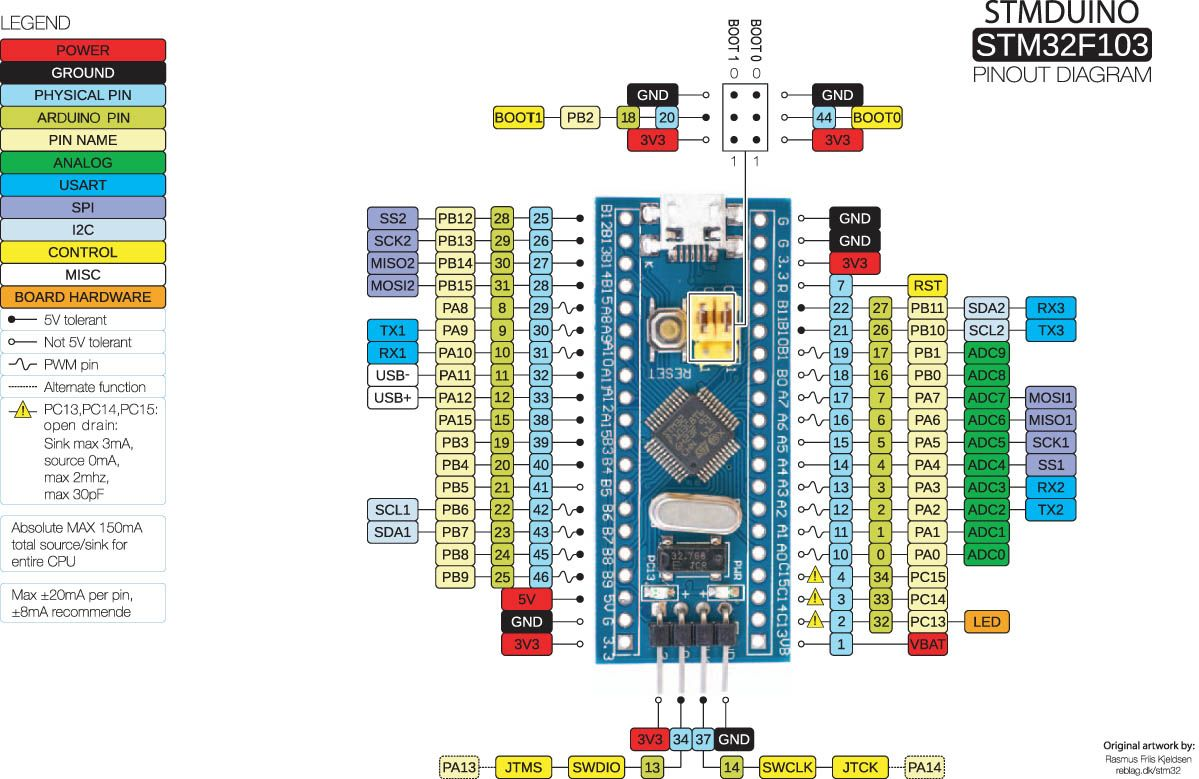
\includegraphics[width=\textwidth]{../images/bluepill_pinout.jpg}
  \caption{Zestawienie pinów mikrokontrolera}
\end{figure}

\section{Akcelerometr}


\chapter{Realizacja programowa - software}
\section{Narzędzia programistyczne}


\listoffigures
\listoftables

\appendix
% appending section

% listing code (example)
\chapter{Kod źródłowy}
\thispagestyle{empty}
% main.c file listed
\newgeometry{a4paper,margin=20mm}
\lstinputlisting[language=C]{../../src/controller_stm32/main.c}
\end{document}
